\section{Desarrollo}

\subsection{Matriz Banda}

Como explicamos en la introducción de la matriz banda, llegamos a la conclusión de que la matriz de ecuaciones de la representación del parabrisas tenía forma de la denominada "matriz banda" cuya respectiva banda era de tamaño m+m+1 con m siendo el ancho del parabrisas. Este es un hecho importante ya que las matrices banda tienen caracteristicas especiales de las cuales es posible la optimización temporal y espacial para resolver el sistema de ecuaciones con eliminación gausseana.

\subsubsection{Optimización espacial}

El problema de representar la matriz original es que la mayoría de los valores son 0 y solo importan los elementos de la banda de la matriz, por lo tanto una forma de optimizar espacialmente es solo guardar la banda, con lo que se logra reducir considerablemente el espacio en esta representación, ya que suponiendo que se tiene un parabrisas de n filas y m columnas, el tamaño de la matriz original sería de $(n*m)^2$, mientras que con la optimización de matriz banda quedaría de tamaño (n*m)*(2*m+1).

El método para construir la representación optimizada de la matriz banda es simple, se guardar la diagonal en una matriz, quedando en el centro los elementos de la diagonal dependiendo de lo que haya en esa posición, ya que en el caso de que sea vacía esta deberá tener coeficientes de las posiciones adyacentes. Además nos dimos cuenta que se podía representar la matriz de tal forma que presente una mejor optimización temporal, y consiste en no poner los coeficientes de las celdas vacias adyacentes si estas no son vacias, en tal caso al vector de resultados le restamos la temperatura de la misma, generando que luego no sea necesario considerar las posiciones no vacias para la eliminación gausseana a la hora de resolver el sistema, y como consecuencia la no necesidad de intercambiar filas al triangular.

\begin{verbatim}

por cada posición del parabrisas //O(N*M)
       pos = fila posicion + columna posicion * ancho;
		
              si en esa posición hay una SANGUIJUELA:
			
                     bandMatrix[pos][ancho] = 1;
                     resultados[pos] = ts;
		
              si esa posición es borde FRIO:
                    
                     bandMatrix[pos][ancho] = 1;
                     resultados[pos] = -100;


              en caso de que esa posición sea VACIA:
                     bandMatrix[pos][ancho] = -4;
                     resultados[pos] = 0;
                    
                     si la izquierda no es vacìa
                            resultados[pos] -= temperatura del de la izquierda;
                     else
                             bandMatrix[pos][ancho-1] = 1;

                    si la de arriba no es vacìa
                            resultados[pos] -= temperatura del de arriba;
                     else 
                            bandMatrix[pos][0] = 1;

                     si la de la derecha no es vacìa
                            resultados[pos] -= temperatura del de la derecha;
                     else 
                            bandMatrix[pos][ancho+1] = 1;
                     
                     si la de abajo no es vacìa
                            resultados[pos] -= temperatura del de abajo;
                     else 
                            bandMatrix[pos][ancho*2] = 1;
		

\end{verbatim}
\subsubsection{Optimización temporal}

Para resolver el sistema de ecuaciones lo que se aplica es una eliminación gausseana optimizada y sin la necesidad de intercambiar filas al momento de generar la matriz triangular superior debido a la optimización que se aplicó en el momento de su creación. La eliminación gausseana fue optimizada teniendo en cuenta la forma de la matriz banda que se genera a partir del parabrisas y conociendo sus caracteristicas, ya que al momento de resolverla detecta cuando la posición es no vacia y no necesita triangular en esa fila debido a que ya sabe que abajo son todos ceros. Por la forma que se almacena la matriz banda lo primero que se hace es triangular en diagonal a la izquierda entre las filas vacias, dando como resultado una matriz triangular superior, luego solo le restará hacer una back substitution optimizada, que consiste en realizar algo parecido a lo anterior pero esta vez de abajo hacia arriba, es decir, resta fila a fila "diagonalizando" y en cada fila que se posicion como sabe que solo tiene un coeficiente igualado a un resultado.

\begin{verbatim}

//PRIMERO LA HAGO TRIANGULAR SUPERIOR
PARA CADA FILA DE LA BANDA, DE ARRIBA A ABAJO
		
   SI NO ES VACIO SE QUE ABAJO HAY TODO CERO, CONTINUO
   SI ES VACIA DIAGONALIZO:
        
         centro = bandMatrix[i][n];
         actual = bandMatrix[i+h][n-h];
         multiplicador = actual / centro;
		
         fila[i+h] - fila[i];

         resultado[i+h] -= resultado[i] * multiplicador;
   

    //BACK SUBSTITUTION
    PARA CADA FILA DE LA BANDA, DE ABAJO A ARRIBA
        fila = i / n;
        for( int h = 1; h <= n; h++){ // COMO ES BANDA ME FIJO SI EN LA DIAGONAL IZQ INF HAY DISTINTO DE 0 PARA PIVOTEAR
           
             centro = bandMatrix[i][n];
             actual = bandMatrix[i-h][n+h];
           
             multiplicador = actual / centro;
		
             fila[i-h] - fila[i];
             resultado[i-h] -= resultado[i]* multiplicador;
                
             lleno el parabrisas con las temperaturas actuales
\end{verbatim}


\subsubsection{Ejemplo}
\begin{figure}[htb]
\begin{center}
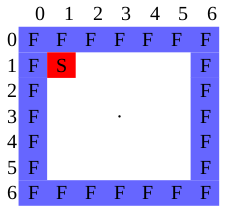
\includegraphics[scale=0.70]{imagenes/parabrisasej.png} 
\caption{Vista de la representación de Parabrisas del ejemplo} 
\end{center}
\end{figure}

\newpage
\begin{figure}[htb]
\begin{center}
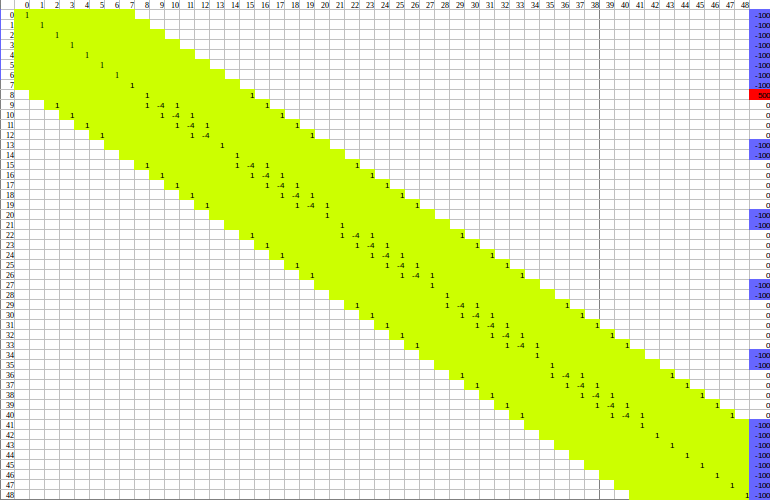
\includegraphics[scale=0.50]{imagenes/matrizej.png} 
\caption{Matriz de ecuaciones del ejemplo} 
\end{center}
\end{figure}

\newpage

\begin{figure}[htb]
\begin{center}
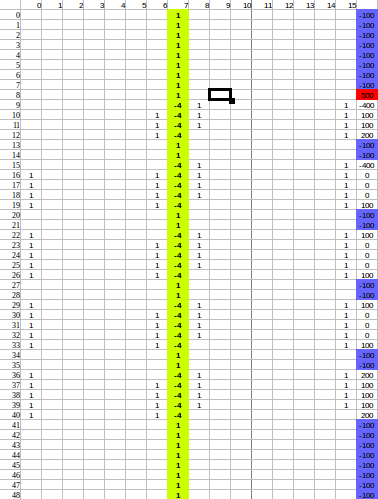
\includegraphics[scale=0.70]{imagenes/matrizbandaej.png} 
\caption{Matriz banda del ejemplo} 
\end{center}
\end{figure}

\newpage

\subsection{Eliminación Gaussiana}
 A modo de comparación recreamos el clásico método de resolución de Eliminación Gaussiana que consta de la eliminación progresiva de variables en el sistema de ecuaciones, hasta tener sólo una ecuación con una incógnita. Una vez resuelta esta, se procede por sustitución regresiva hasta obtener los valores de todas las variables.

\begin{verbatim}
Class Windshield{
    resolveByGaussianElimination(){
         gaussianElimination();
         backSubstitution();
    } 
    gaussianElimination(){
        for rows k already been reduced
            iMax = findPivot();
            Swap rows k and imax;
            Force 0’s in column A[k+1..n-1][k];
    }
    backSubstitution(){
        for row from last to first:
            calculateFromNextOneExceptForLast()
    }
}
\end{verbatim}



\subsection{Soluciones}

Para resolver el problema que se nos pide, planteamos distintos tipos de solución. Inicialmente encaramos el problema de manera exacta, pero lo deshechamos inmediatamente ya que sabiendo que es un problema de decisión, el tiempo para determinar cuál es el número mínimo de sanguijuelas a eliminar es exponencial en la cantidad de estas. Es por eso que decidimos realizar una heurística, ya que el tiempo es preciado cuando el parabrisas de nuestra nave tiene poco tiempo antes de que se rompa en caso de estar en situación crítica. Para modo de comparación tomamos dos tipos de algoritmos para establecer que es una mejor solución.


\subsection{Solución Greedy + Local Search}
Esta solución consiste, a grandes rasgos, en ir matando las sanguijuelas del medio (ya que son las que mayor temperatura generan en el punto crítico) hasta que el punto central este por debajo del 235 Cº. Finalmente, tratar de realizar una búsqueda local intentado volcar de vuelta en el parabrisas sanguijuelas que habíamos decidido sacar y viendo si era realmente necesario eliminarla para poder salir del estado crítico. La decisión de hacer LocalSearch está dada para el caso de que exista una sanguijuela en el centro y dos a la misma distancia. Pero de un lado haya una linea de muchas sanguijuelas, por lo que es muy probable que con sacar la del lado de la linea fuera suficiente. A continuación podemos observar el resultado de lo recién descripto. Inicialmente había una sanguijuela en el medio y una equidistante a la que quedó, pero eligió sacar esta del lado de la linea.

\begin{figure}[htb]
\begin{center}
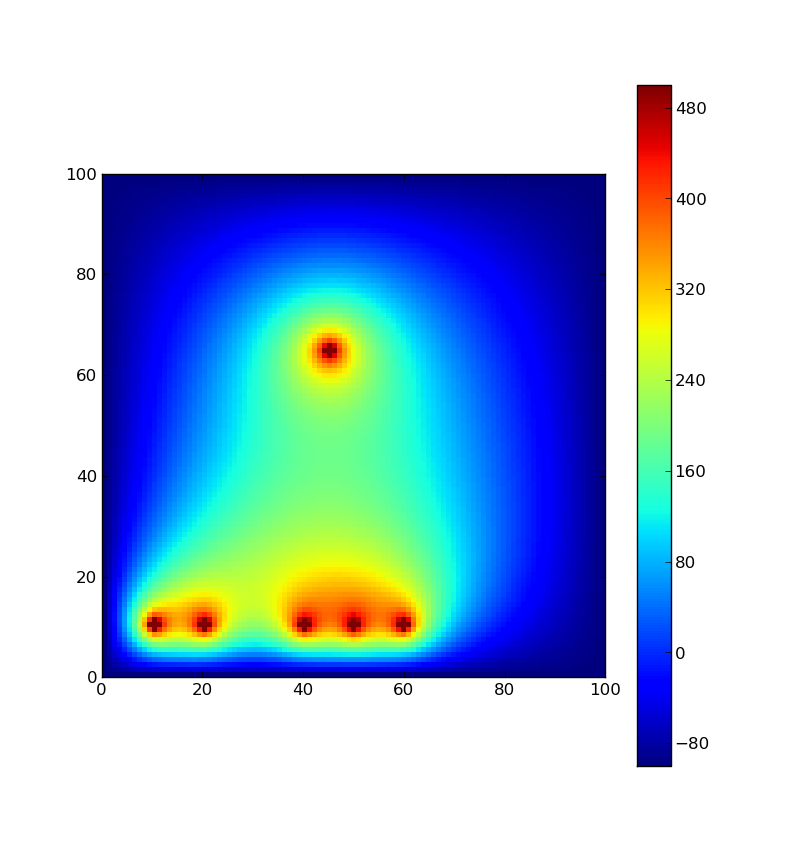
\includegraphics[scale=0.50]{imagenes/greedy_corrido.png} 
\caption{Resultado tercer corrida} 
\end{center}
\end{figure}

\newpage
Pseudocodigo:

\begin{verbatim}
Class Windshield{
    greedySolution(){
        orderLeachesByDistanceToCenter()
         while(!this->isCooledDown(){
             leachesToRemove(this->removeFirstNotRemovedLeachOrderedCentrically())
         }

         localSearchTryToReturnLeaches(leachesToRemove);

         return leachesToRemove;
    } 
    isCooledDown(){
         recalculateByBandMatrix();
         return (matrix.centerPoint < Ts)
    }
    orderLeachesByDistanceToCenter(){
        sort(leaches).by(lambda {|leach,otherLeach| leach.distanceToCenter < otherLeach.distanceToCenter})
    }

    localSearchTryToReturnLeaches(leachesToRemove){
        for (leach in leachesToRemove){
            putBackLeachInWindshield(leach);
            if (isCooledDown){
                leachesToRemove.erase(leach)
            }else{
                takeOutLeachFromWindshield(leach);
            }
        }
    }
}
\end{verbatim}



\subsection{Solución Random}\label{sec:solucionRandom}


En esta solución seleccionamos de nuestro array de posiciones de sanguijuelas (que es el array recibido por parametro, osea con las posiciones sin discretizar) una al azar y la eliminamos. Luego ejecutamos de nuevo el cálculo de las temperaturas y chequeamos si el punto crìtico esta por debajo del 235 Cº.Si no lo está, elegimos otra al azar y repetimos el proceso hasta que lo esté. 

Pseudocodigo:

\begin{verbatim}
Class Windshield{
    randomSolution(){
         while(!this->isCooledDown(){
             this->randomKill()
         }
    } 
    isCooledDown(){
         return (matrix.centerPoint < Ts)
    }
    randomKill(){
         randomRemove(posSanguijuelas)
         this->recalculateTemps()
    }
}
\end{verbatim}

Vale aclarar que el recalculateTemps utiliza el metodo band matrix, ya que este es màs rápido.









